\section{实验2:AI在多产品场景中的中性广告个性化生成能力}
基于实验1的结果,AI生成的个性化广告在宜人性和外倾性两个维度上表现出较好的效果,而针对尽责性和神经质个体设计的个性化广告未能达到显著效果。此外,针对开放性个体设计的个性化广告虽呈现边缘显著的效果,但其影响仍需进一步检验。这表明,尽管AI具备生成个性化广告的能力,其在不同人格特质群体中的适配性仍存在差异。因此,实验2进一步探讨AI在个性化广告生成中的表现,尤其关注在实验1中未达到显著效果的\textbf{尽责性}和\textbf{开放性} 维度,以考察AI是否能够为这些人格特质设计更具针对性的个性化广告。此外,实验2在AI生成广告的研究框架上引入了另一关键因素:\textbf{产品本身}。产品不仅承载了核心营销信息,还影响了广告文本的内容和个性化策略。在实验1中,研究采用手机这一中性产品,以尽可能减少产品类型对个性化广告效果的潜在干扰。然而,在实际广告创作中,不同产品可能具有不同的消费者认知框架与个性化需求。因此,实验2进一步扩展研究范围,考察AI在不同产品场景下的个性化广告生成能力,以验证其是否能够适应多样化产品类别,并针对不同人格特质有效调整广告文本。除此之外,实验2还考察AI在\textbf{中性广告基础上进行个性化改写}的能力。相比于从零生成个性化广告,许多广告实践中更常见的做法是基于已有的广告文本进行调整,使其更符合特定目标受众的个性化需求。因此,本研究采用来自社交媒体的真实中性广告作为基础文本,并通过AI生成针对不同人格特质的个性化版本,以评估AI在广告内容调整与定向优化方面的能力。

本实验采用 \textbf{GPT-4} 作为广告生成模型,相较于实验1使用的GPT-3.5,GPT-4在理解与生成复杂文本方面具有更强的能力,从而进一步提高个性化广告的质量与针对性。通过引入多产品场景与中性广告改写的任务,实验2旨在更全面检验AI在真实广告创作环境中的个性化生成能力。

为设计实验条件并选择适合的产品类型,我们参考了享乐型产品与实用型产品的经典区分 \citep{crowley1992measuring}。根据定义,享乐型产品(hedonic products)指那些主要满足消费者感官愉悦和情感体验的产品,其核心价值体现在提供的快感和享受感,如甜点、香水或娱乐活动。相对而言,实用型产品(utilitarian products)更强调功能性和实用性,其核心价值在于满足消费者的实际需求,如厨房用具、办公设备或清洁用品。结合人格特质的经典定义 \citep{john1991big} 和产品价值理论 \citep{dhar2000consumer} 可以发现,享乐型产品(hedonic products)本质上与快感和感官满足相关,能够为消费者提供愉悦和情感上的满足。因此,它们更符合高开放性个体的偏好,这类个体倾向于追求新体验和情感深度,表现出对创造性和探索性的强烈需求。而实用型产品(utilitarian products)以功能性和效率为核心价值,更容易吸引高尽责性个体,这类个体通常注重组织性、责任感和目标导向。已有研究也支持了这一人格与产品价值的匹配关系 \citep{guido2006shopping,huang2010relationship}。

基于以上理论,我们选择享乐型和实用型产品作为实验场景,并以尽责性和开放性作为目标个性化特质。本实验的核心问题在于:\textbf{AI是否能够在不同产品场景下表现出一致且稳定的个性化生成能力?} 换言之,我们关注AI是否能够跨越产品类别,生成符合目标人格特质的个性化广告内容。此外,本实验还开放性探讨个性化效果是否会受到特质与产品之间匹配效应的影响。例如,针对高开放性个体定制的个性化广告是否在享乐型产品中比在实用型产品中更有效?针对高尽责性个体定制的个性化广告是否在实用型产品中比在享乐型产品中更有效?

\subsection{方法}
\label{study1-substudy2-methods}

本实验采用 \textbf{2(广告类型:享乐/实用) × 2(人格特质:尽责性/开放性)} 的被试内设计。针对每一产品与人格特质的组合,均包含一个来源于社交媒体的中性广告和一个基于该中性广告生成的个性化广告。每名被试需依次观看每组广告(共四组),广告呈现顺序随机,并对每组广告进行评价。

\textbf{(1)被试}

通过见数平台发布实验,154名参与者自愿参加这项研究。11名参与者由于注意检查测试未通过被剔除,剩余\textbf{143}名有效被试(年龄范围= 18-55岁;\textit{M}=25.97岁;\textit{SD}=7.30;女性101名)。参与任务的每名参与者获得2元人民币作为报酬。注意力检测包含两部分:一是因变量测量中嵌入的明确指令题(如“请选2”);二是问卷末尾关于广告产品的识别题,要求参与者从薯片、电脑、手机、香氛和牙膏中正确选择广告涉及的两项(电脑和薯片)。


\textbf{(2)实验材料:广告设计}

本实验材料包括两种类型的广告材料:中性广告和基于中性广告生成的个性化广告。实验首先确定目标产品,通过社交媒体筛选中性广告,并利用GPT-4生成个性化广告。

在产品选择阶段,为区别享乐型与实用型产品,我们进行了前测实验,邀请了135名参与者对18种商品进行分类(如冰淇淋、薯片、电影票、电脑、牙膏等),这些商品的选择基于前人文献\citep[如][]{huettl2012visual} 中提到的享乐型和实用型产品。参与者被告知享乐型产品 (\textit{能够带来愉悦和幸福但非必需的商品})和实用型产品(\textit{以功能性和实用性为核心,具有实际用途})的定义,并对每件商品进行分类。结果显示,绝大多数参与者将“薯片”归类为享乐型产品(97.78\%),而将“电脑”归类为实用型产品(96.30\%)。因此,本实验选择薯片和电脑分别作为享乐型与实用型产品的代表。

确定目标产品后,我们选择了与目标产品匹配的知名品牌作为参考:薯片选择「乐事」(Lay’s),电脑选择「戴尔」(Dell)。随后,在这些品牌的官方社交媒体账号(如微博和小红书)上收集相关广告。广告内容分为文本和图片两部分。在提取广告文本时,我们删除了所有涉及品牌名称或标识的信息;在选择广告图片时,优先使用未包含品牌logo的图片版本,以避免品牌效应对实验的潜在影响。

基于这些中性广告,我们利用GPT-4生成个性化广告。具体方法是以中性广告的文本内容为基础,输入GPT-4有关个性化生成的提示语,指导其生成针对高开放性和高尽责性个体的定制广告。提示语(详见附录)包括明确的个性化生成指令、相关人格特质的定义(与实验1一致)以及中性广告的文本内容。每个目标产品生成两则个性化广告,分别针对开放性和尽责性,最终为每个产品设计了三种广告版本(一个中性广告、两个个性化广告)。为增强实验情境的真实性和生态效度,所有广告均以模拟微博帖子形式呈现(如图 \ref{fig:Study1-exp2-ads},其他完整内容详见附录)。每则广告均使用虚构品牌名“X薯片”和“X电脑”,并包含产品图片和文字说明。针对同一产品的广告保持图片内容一致,但文本内容根据中性或人格定制的要求有所不同。此外,广告中还包含模拟社交媒体的互动元素(如点赞、评论和分享按钮),以进一步提升实验情境的真实性。

\begin{figure}[H]
    \centering
    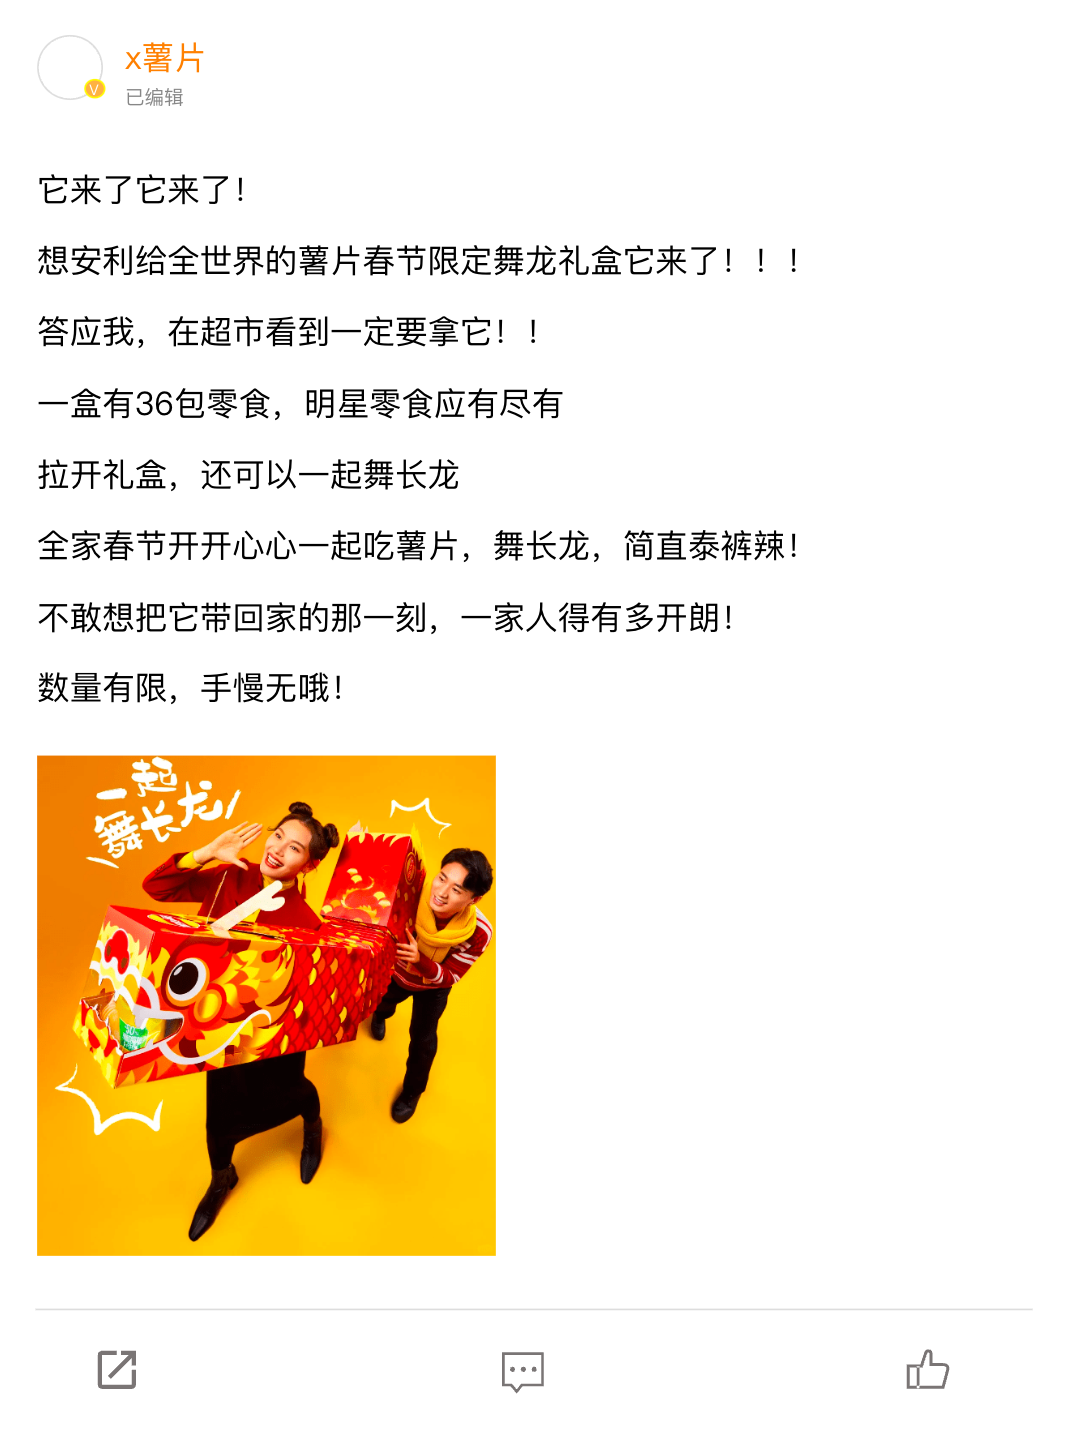
\includegraphics[width=.3\linewidth]{Image/Study1-exp2-ads.png}
    \caption{\label{fig:Study1-exp2-ads}实验开始前的广告示意图}
\end{figure}

为在正式实验前验证个性化广告的有效性,本研究通过见数平台发布预实验,共有60名参与者自愿参加,完成实验后获得1元人民币作为报酬。每名参与者需对2种产品(薯片和电脑)* 3种广告(中性广告和两种个性化广告)进行评价。评分方式与实验1b的预实验一致。参与者需围绕广告的目标消费者特点对广告进行评分,采用1-5点李克特量表,其中1分表示更符合“低水平”描述,5分表示更符合“高水平”描述。例如,对于针对高尽责性设计的广告,参与者需基于以下特征进行评分,从“粗心的、容易分心的、不拘小节的、做事缺少条理的”到“可靠的、有组织的、自律的、注重细节的、有条理”。预实验结果表明(如表\ref{tab:study1-exp2-pretest-results}),生成的个性化广告有效。与中性广告相比,个性化广告在更大程度上符合目标消费者的特点。

\begin{table}[H]
    \centering
    \caption{\label{tab:study1-exp2-pretest-results} 预实验结果:个性化广告与中性广告评分均值}
    {\tablesongti % 整个表格环境应用宋体六号字体
    \renewcommand{\arraystretch}{1} % 调整行距
    \begin{tabular}{l c c c}
        \toprule
        \textbf{产品} & \textbf{目标个性特质} & \textbf{个性化广告(均值)} & \textbf{中性广告(均值)} \\
        \midrule
        薯片 & 尽责性 & 3.82 & 3.47 \\
        薯片 & 开放性 & 3.94 & 3.70 \\
        电脑 & 尽责性 & 4.07 & 3.57 \\
        电脑 & 开放性 & 4.12 & 3.78 \\
        \bottomrule
    \end{tabular}
    }
\end{table}


\textbf{(3)问卷测量}

a. 大五人格量表。因本实验聚焦开放性和尽责性两个维度,我们从\citet{john1991big}编制44道题目的大五人格量表中筛选对应特质的题目。其中,开放性对应10个题项,尽责性对应9个题项。参与者对每个题项的回答均采用1-5点李克特量表,1分表示“完全不符合”,5分表示“完全符合”。

b. 广告说服效果。实验中,每组中性广告和对应的个性化广告以并排形式随机呈现,分别标记为广告A和广告B。参与者需对两则广告的偏好进行评分,评分采用5点双极量表(如图\ref{fig:study1-exp2-rating-example}),分值范围从“更倾向于广告A”到“更倾向于广告B”。为统一结果解读,分数在统计时进行转换,使得分数越高表示越偏好个性化广告,分数越低表示越偏好中性广告。具体的题项与实验1一致(详见 \ref{study1-substudy1-measurement},包含五个题项,用于评估参与者对广告和产品的态度以及购买意图。每个题项均采用1-5点李克特量表评分,广告说服效果的总评分为五个题项得分的平均值。

\begin{figure}[H]
    \centering
    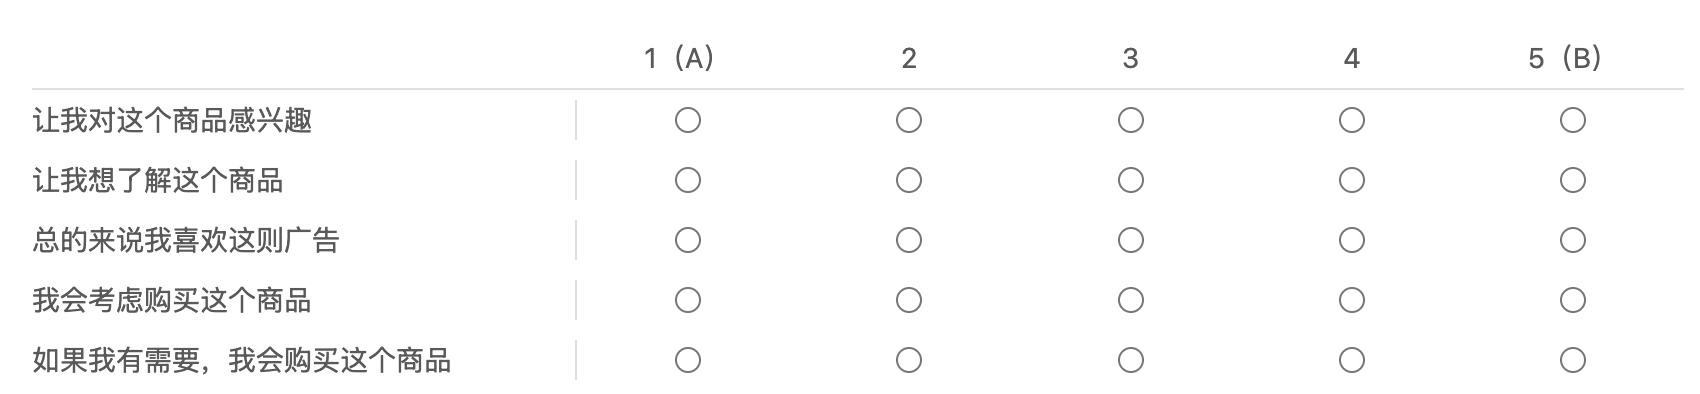
\includegraphics[width=.7\linewidth]{Image/Study1-exp2-rating.png}
    \caption{\label{fig:study1-exp2-rating-example}实验评分示意}
\end{figure}



\subsection{实验流程}
本实验的流程分为两个部分。第一部分,参与者依次阅读每组广告(个性化广告与中性广告并排呈现),并对每组广告的相对说服效果进行评分。广告呈现顺序随机化,以控制顺序效应。第二部分,参与者需回答与人格测试相关的问卷题目,最后提供年龄、性别等人口统计学信息。

\subsection{结果}
我们分别对尽责性个性化广告和开放性个性化广告进行了回归分析。回归模型的自变量包括参与者对应人格特质的得分(尽责性/开放性)、产品类型(电脑/薯片)以及特质与产品类型的交互项,因变量为广告的说服效果。由于评分为二极分布,我们对数据进行了转换,使得得分越高表示相较于中性广告,参与者对个性化广告的偏好越强。

针对尽责性个性化广告,回归模型如下: \begin{equation} Y_{\text{尽责性}} = \beta_0 + \beta_1 \cdot \text{尽责性特质} + \beta_2 \cdot \text{产品类型} + \beta_3 \cdot (\text{尽责性特质} \times \text{产品类型}) + \epsilon \end{equation}

回归分析结果显示,\textbf{尽责性特质的主效应显著}(\textit{$\beta$} = 0.3455, \textit{p} = 0.038),但产品类型的主效应(\textit{$\beta$} = 0.8079, \textit{p} > 0.05)和特质与产品类型的交互项(\textit{$\beta$} = -0.1372, \textit{p} > 0.05)均不显著。这表明,尽责性得分较高的个体相较于中性广告,更偏好针对高尽责性设计的个性化广告,但这种偏好不因产品类型而显著变化。

针对开放性个性化广告,回归模型如下: \begin{equation} Y_{\text{开放性}} = \beta_0 + \beta_1 \cdot \text{开放性特质} + \beta_2 \cdot \text{产品类型} + \beta_3 \cdot (\text{开放性特质} \times \text{产品类型}) + \epsilon \end{equation}

回归分析结果显示,\textbf{开放性特质的主效应显著}(\textit{$\beta$} = 0.3349, \textit{p} = 0.048),但产品类型的主效应(\textit{$\beta$} = -0.9128, \textit{p} > 0.05)和特质与产品类型的交互项(\textit{$\beta$} = 0.1851, \textit{p} > 0.05)均不显著。这表明,开放性得分较高的个体相较于中性广告,更偏好针对高开放性设计的个性化广告,同样,这种偏好不因产品类型的不同而显著变化。